% !TEX TS-program = pdflatex
% !TEX encoding = UTF-8 Unicode

% TeX-CS (version 1.0)
% For Computer Science classes at the University of Texast at Austin
% Notes template created by Abdon Morales for the College of Natural Science
% and for the Department of Mathematics and Computer Science
% (c) 2024 Abdon Morales and the University of Texas at Austin
% This is a notes template for a LaTeX document using the "article" class for Mathematics (Calculus)
% at the University of Texas at Austin.

% Last change made: Feb 8, 2024 12:45 AM CST


% See "book", "report", "letter" for other types of document.

\documentclass[11pt]{article} % use larger type; default would be 10pt

% Start of Article customization options and addons (for more help and information reference to Overleaf's guides and docs on Latex.
\usepackage[utf8]{inputenc} % set input encoding (not needed with XeLaTeX)

%%% Examples of Article customizations
% These packages are optional, depending whether you want the features they provide.
% See the LaTeX Companion or other references for full information.


%%% PAGE DIMENSIONS
\usepackage{geometry} % to change the page dimensions
\geometry{letterpaper} % or letterpaper (US) or a5paper or....
% \geometry{margin=2in} % for example, change the margins to 2 inches all round
% \geometry{landscape} % set up the page for landscape
%   read geometry.pdf for detailed page layout information

\usepackage{graphicx} % support the \includegraphics command and options
\usepackage{xcolor}

% \usepackage[parfill]{parskip} % Activate to begin paragraphs with an empty line rather than an indent


%%% PACKAGES
\usepackage{booktabs} % for much better looking tables
\usepackage{array} % for better arrays (eg matrices) in maths
\usepackage{paralist} % very flexible & customisable lists (eg. enumerate/itemize, etc.)
\usepackage{verbatim} % adds environment for commenting out blocks of text & for better verbatim
\usepackage{subfig} % make it possible to include more than one captioned figure/table in a single float

%%% Math tools for Computer Science
\usepackage{mathtools}
\usepackage{amsmath}
\usepackage{tikz} % For charts, mathematical graphs, and etc
\usepackage{tcolorbox}
%% Equal symbol for L'Hospital Rule
\usepackage{tcolorbox}
\newcommand\LR{\stackrel{\mathclap{\normalfont\mbox{L.R}}}{=}}

% Encoding.
\usepackage[T1]{fontenc}

% Font.
\usepackage{ccfonts,eulervm}
\usepackage{dsfont}
% Spaces.
\usepackage{xspace}

% Parser.
\usepackage{xparse}

% Language.
\usepackage[english]{babel}

% Math.
\usepackage{amsthm}

% Symbols.
\usepackage{amssymb}
\usepackage{wasysym}
\usepackage{textcomp}

% Graphics.
\usetikzlibrary{shapes, patterns, positioning}
\usepackage{subcaption}

% Hyperlinks.
\usepackage[
	colorlinks=true
]{hyperref}

% References.
\usepackage[
	sort&compress,
	nameinlink,
	noabbrev
]{cleveref}

% Quotations.
\usepackage{csquotes}

% Bibliography.
\usepackage[
	backend=biber,
	style=numeric,
	natbib=true,
	hyperref=true,
	date=year,
	sortcites=true,
	maxbibnames=50,
	maxcitenames=2,
	firstinits=true,
	isbn=false,
	url=false,
	doi=false
]{biblatex}

% Bucketlist.
\usepackage{todonotes}

% These packages are all incorporated in the memoir class to one degree or another...

%%% Doc and Math macros

% Structure.
\theoremstyle{plain}
\newtheorem{theorem}{Theorem}
\newtheorem{proposition}[theorem]{Proposition}
\newtheorem{corollary}[theorem]{Corollary}
\newtheorem{lemma}[theorem]{Lemma}

\theoremstyle{definition}
\newtheorem{definition}[theorem]{Definition}
\newtheorem{simulation}[theorem]{Simulation}
\newtheorem{observation}[theorem]{Observation}
\newtheorem{conjecture}[theorem]{Conjecture}

% Abbreviations.
\newcommand{\ie}{i.e.\xspace}
\newcommand{\etal}{et al.\xspace}
\newcommand{\etc}{etc.\xspace}
\newcommand{\eg}{e.g.\xspace}
\newcommand{\fig}{fig.\xspace} % figure
\newcommand{\vv}{v.v.\xspace} % vice versa

% Basics.
\newcommand{\on}[1]{\operatorname{#1}}
\newcommand{\defas}[0]{\mathrel{\mathop:}=} % define as
\newcommand{\asdef}[0]{=\mathrel{\mathop:}} % as defined
\newcommand{\ddd}[0]{, \ldots, } % , ..., 

% Logic.
\newcommand{\fa}[0]{~\forall}
\newcommand{\st}[0]{\mathrel{:}} % such that
\newcommand{\is}[0]{\mathrel{:}}
\newcommand{\from}[0]{\mathop{~:~}}

% Sets.
\newcommand{\set}[1]{\left\{#1\right\}}
\newcommand{\nin}[0]{\not\in}
\newcommand{\with}[0]{\mathrel{|}}
\newcommand{\powerof}[1]{\mathcal{P}\left(#1\right)} % P(Set)
\newcommand{\power}[1]{2^#1} % 2^Set
\newcommand{\len}[1]{\ensuremath{|#1|}}
\newcommand{\eset}[0]{\emptyset}

% Numbers.
\newcommand{\N}[0]{\mathbb{N}}
\newcommand{\Z}[0]{\mathbb{Z}}
\newcommand{\Q}[0]{\mathbb{Q}}
\newcommand{\R}[0]{\mathbb{R}}
\newcommand{\onerange}[1]{\{1 \ddd #1\}}
\newcommand{\zerorange}[1]{\{0 \ddd #1\}}

% Functions.
\newcommand{\sign}[0]{\on{sign}}
\newcommand{\norm}[1]{\lVert #1 \rVert}
\newcommand{\cif}[0]{\text{, if }}
\newcommand{\els}[0]{\text{, otherwise}}

% Probability.
\newcommand{\prob}[1]{\mathrm{P}(#1)}
\newcommand{\expected}[1]{\mathrm{E}[#1]}
\newcommand{\given}[0]{\mathrel{|}}

% Complexity.
\renewcommand{\O}[0]{\ensuremath{\mathcal{O}}} % Big-O-Notation
\newcommand{\p}[0]{\ensuremath{\text{P}}}
\newcommand{\np}[0]{\ensuremath{\text{NP}}}
\newcommand{\rp}[0]{\ensuremath{\text{RP}}} % Randomized polynomial time
\newcommand{\bpp}[0]{\ensuremath{\text{BPP}}} % Bounded-error prob. polynomial time
\newcommand{\zpp}[0]{\ensuremath{\text{ZPP}}} % Zero-error prob. polynomial time
\newcommand{\nphard}[0]{\ensuremath{\np\text{-hard}}} % NP-hard
\newcommand{\npcomplete}[0]{\ensuremath{\np\text{-complete}}} % NP-complete


%%% HEADERS & FOOTERS
\usepackage{fancyhdr} % This should be set AFTER setting up the page geometry
\pagestyle{fancy} % options: empty , plain , fancy
\renewcommand{\headrulewidth}{0pt} % customise the layout...
\lhead{}\chead{}\rhead{}
\lfoot{}\cfoot{\thepage}\rfoot{}


%%% SECTION TITLE APPEARANCE
\usepackage{sectsty}
\allsectionsfont{\sffamily\mdseries\upshape} % (See the fntguide.pdf for font help)
% (This matches ConTeXt defaults)


%%% ToC (table of contents) APPEARANCE
\usepackage[nottoc,notlof,notlot]{tocbibind} % Put the bibliography in the ToC
\usepackage[titles,subfigure]{tocloft} % Alter the style of the Table of Contents
\renewcommand{\cftsecfont}{\rmfamily\mdseries\upshape}
\renewcommand{\cftsecpagefont}{\rmfamily\mdseries\upshape} % No bold!

%%% The "real" document content comes below...

\title{Economic Growth and the Wealth of Nations}
\author{Abdon Morales \\ The University of Texas at Austin \\ ECO 304L \\ Wayne Geerling}
\date{\today \\ Chapter 11 : Week 5}
%\date{} % Activate to display a given date or no date (if empty),
         % otherwise the current date is printed 

\begin{document}
\maketitle
\subsection*{There's more to prosperity than natural resources}

Many people believe that natural resources, such as trees, oil, and farmland, are the primary sources of economic growth. They believe that nations like the United States and Australia are prosperous because these nations have vast natural resources to use in the production of goods and services. A variation on this idea emphasizes geography: nations with the best shipping locations and mildest climates have more prosperous economies.

Striving for economic growth is not only about accumulating more wealth. Yes, economic growth brings smartphones and Jet Skis, but it's much more important than that; economic growth offers the potential for more women and infants to survive childbirth, more people to have access to clean water and better sanitation, and more people to live healthier, longer, and more educated lives.

In this chapter, we begin by looking at the implications of economic growth for human welfare; we then consider the impact of an economy's resources and technology on economic growth. Finally, we discuss the key elements an economy needs in order to grow.
\begin{tcolorbox}[width=\textwidth,colback={white},title={Big Questions},colbacktitle=yellow,coltitle=blue]
\begin{itemize}
\item Why does economic growth matter?
\item How do resources and technology contribute to economic growth?
\item What institutions foster economic growth?
\item How are some economists testing new ideas?
\end{itemize}
\end{tcolorbox}

\newpage

\section*{Why do economic growth matter?}
In 1900, life expectancy in the United States was 47 years; about 140 of every 1,000 children died before their first birthday. Only about one-third of American homes had running water and income [in 2021 dollars] was less than \$ 5,500 per person. Most people lived less than a mile from their job and almost nobody owned an automobile. Yes, this is also a description of life in low-income countries today. What happened in the United States in the meantime? Economic growth!
In this section, we examine how economic growth affects the lives of people around the world. We also examine the historical data on economic growth and explain some mathematics.
\subsection*{Some ugly facts}
Before looking at data on growth, we need to recall how economists measure economic growth. In Chapter 6, we defined \textbf{economic growth} as the percentage change in real per capita GDP. We know that real per capita GDP measures the average level of income in a nation. For most people, life is not all about the pursuit of more income; however, economic growth does alleviate human misery and lengthen lives. Wealthier societies provide better living standards, which include better nutrition, educational opportunities, healthcare, freedom, and even sources of entertainment.

Let's look around the world and compare life in low-income countries. Table 11.1 presents human welfare indicators for some of the world's highest- and lowest-income nations in 2020. Among the low-income nations are Afghanistan, Ethiopia, North Korea, Liberia, Niger, Syria, and Yemen. The high-income nations include Australia, Denmark, Israel, Japan, Germany, South Korea, and the United States.

\begin{center}
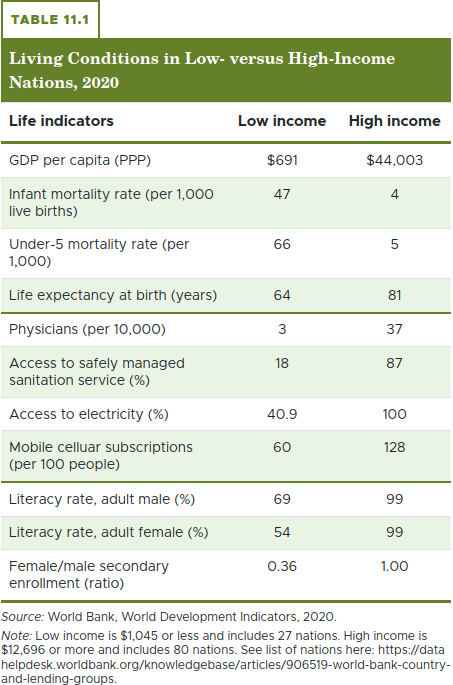
\includegraphics[scale=0.5]{../../images/Chapter 11/table 11.1.png}
\end{center}

The data in Table 11.1 support the contention that per capita GDP matters - not for the sake of more income per se, but because it correlates with better human welfare conditions, which matter to everyone.

\subsection*{Learning from the past}

We can learn a lot about the roots of economic growth by considering the past; historically, a common person's life focused on subsistence, simply trying to find enough food, shelter, and clothing to survive. As we saw in the previous section, even today many people still live on the margins of subsistence; what can history tell us about how high -income nations achieved economic development? This answer will help clairfy possible policy alternatives.

\subsubsection*{We were all poor once}
When you look around the globe today, you see rich nations and poor nations; you can probably name many rich nations: the United States, Japan, Taiwan, and the Western European nations, among others. You might also know the very poor nations: much of Africa, parts of Latin America, and significant parts of Asia; but the world was not always this way. If we consider the longer history of humankind, only recently did the incomes of common people rise above subsistence level.

The Industrial Revolution, during which many economies moved away from agriculture and toward manufacturing in the 1800s, is at the very center of the big increase in world income growth. Beginning with the Industrial Revolution, the rate of technical progress increased so rapidly, it was able to outpace population growth. The foundation for the Industrial Revolution was laid in the preceding decades, and these foundations included private property protection and several technologies innovations. We don't claim that the Industrial Revolution was idyllic for those who lived through it, but legal and other institutional innovations of that era paved the way for the unprecedented gains in human welfare that people have since experienced.
\begin{center}
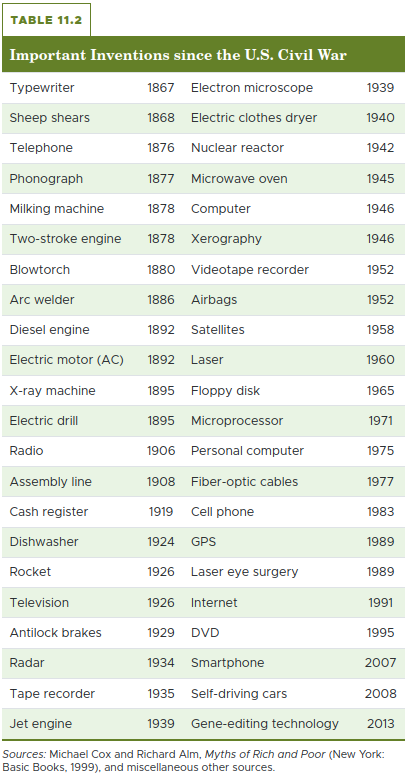
\includegraphics[scale=0.5]{../../images/Chapter 11/table 11.2.png}
\end{center}

This data do not imply that life is always easy and predictable comfortable for everyone in the modern world, but opportunities for the average person alive today are very different from those for the average person alive today are very different from those for the average person in past centuries. Table 11.2 lists a sampling of some of the major innovations of the past century and a half. Try to imagine life without any of these, and you'll get a sense of the gains we've made since the Industrial Revolution.

\subsubsection*{Some got rich, others stayed poor}

Although wealth has increased over the past two centuries, it is not evenly distributed around the globe. Figure 11.2 shows real per capita GDP (in 2020 U.S dollars) for various world regions. In 1820, the income of the average U.S citizen \$ 3,160, or about \$ 9 per day. Imagine trying to live  on \$ 9 per day in today's world - that is, \$ 9 to buy all the food, clothing, shelter, education, transportation, and anything else you might need to purchase. That was life in the United States in 1820, but it also describes the plight of many people in the world today.

\begin{center}
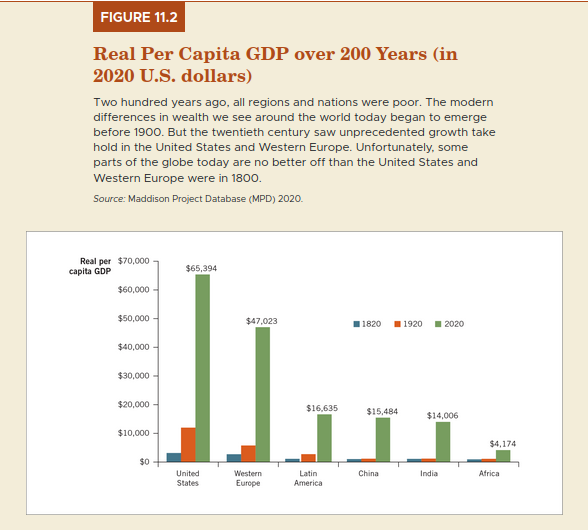
\includegraphics[scale=0.5]{../../images/Chapter 11/Figure 11.2.png}
\end{center}

While many of the current disparities between nations began about 200 years ago, some nations have moved from poor to rich as recently as the past few decades.

\subsection*{Measuring Economic Growth}

Overall, people today are much wealthier than they were 200 years ago; however, this properity did not occur overnight. Rather, income grew a little bit each year; there is a striking mathematical truth about growth: small difference in growth rates lead to large differences in wealth levels over time.  In this section, we explain how economic growth rates are computed, and we consider the level of growth a nation needs for its population to experience significant improvements in living standards.

\subsubsection*{The Mathematics of growth rates}

\begin{center}
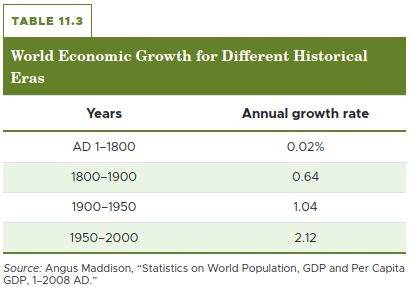
\includegraphics[scale=0.5]{../../images/Chapter 11/table 11.3 .png}
\end{center}

We have seen that economic growth is the annual growth rate of real per capita GDP. It is our measure of how an average person's income changes over time, including an allowance for price changes; but the government reports overall GDP data in nominal terms. Therefore, to get an accurate growth rate, we need to account for both inflation and population growth; we can use the following equation to approximate economic growth, where \(\% \Delta\) indicates the percentage change in a variable:
\begin{equation}
\text{economic growth} \approx \% \Delta \text{in nominal GDP}-\% \Delta \text{price level} - \% \Delta \text{population}
\end{equation}

A word of caution about terminology is in order. There's a big difference between nominal GDP growth, real GDP growth, and real per capita GDP growth. (In Table 11.4, these terms appear in orange.); but sloppy economic reporting sometimes confuses the terms. You may read something like "the U.S economy grew by 2.3\% in 2019," which refers to real GDP growth and is not calculated on a per capita basis; it would be an even bigger mistake to claim that U.S economic growth in 2019 was 4.1\% , a number not adjusted for either population growth or inflation. Such confusing wording is a common mistake in reports on international economic growth statistics.

\begin{center}
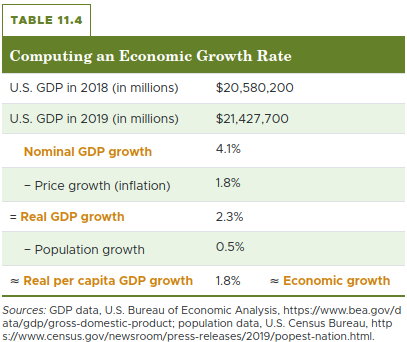
\includegraphics[scale=0.5]{../../images/Chapter 11/table 11.4 .png}
\end{center}

\subsubsection*{Growth rates and income levels}

Before we consider policies that might aid economic growth, we need to look more closely at how growth rates affect income level.

First, consider how significant it is when income doubles, or increases by 100\%. If your income doubled today - all else being equal - you could afford twice as much of everything you are currently buying. Now imagine what would happen if income doubled for an entire country or even for all countries. In the United States, real per capita GDP doubled in the 40 years between 1980 and 2020. This means that the average person living in the United States now can afford twice as much food, clothing, transportation, education, and even government services as the average U.S resident in 1980; that's quite a difference.

But increasing real income by 100\% in a single year is not realistic; let's use an annual growth rate closer to reality - say, 2\%, which has historically been an average rate of economic growth for the United States. With 2\% annual growth, how long does it take to double your income?

Table 11.5 illustrates the process of compounding over time by showing the increase from year to year.

\begin{center}
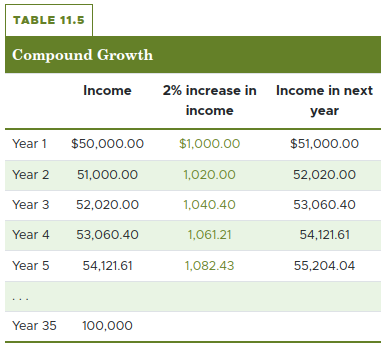
\includegraphics[scale=0.5]{../../images/Chapter 11/Table 11.5.png}\\
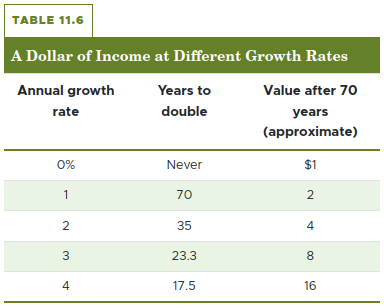
\includegraphics[scale=0.5]{../../images/Chapter 11/Table 11.6.png}
\end{center}

\subsubsection*{The Rule of 70}

We saw that when income grows at 2\% per year, it doubles in approximately 35 years. A simple rule known as the \textbf{rule of 70} determines the lenght of time necessary for a sum of money to double at a particular growth rate. According to the rule of 70: \textit{If the annual growth rate of a variable x\% , size of that variable doubles approximately every \(70 \div \text{x years}\).}

The rule of 70 is an approximation, but it works well with typical economic growth rates.

Table 11.6 illustrates the rule of 70 by showing how long it takes for a single dollar of income to double in value, given different growth rates.

The rule of 70 shows us that small and consistent growth rates, if sustained for a decade or two, can greatly improve living standards. Over the long course of history, growth rates were essentially zero, but the past two centuries have seen small, consistent growth rates, and the standard of living for many has increased dramatically.

We can look at actual growth rates of various countries over a long period to see the impact on income levels. Table 11.7 presents growth rates of several countries over the 66 years from 1950 to to 2016.

\begin{center}
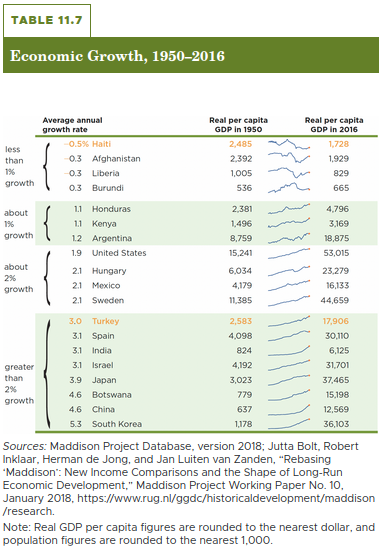
\includegraphics[scale=0.5]{../../images/Chapter 11/Table 11.7 .png}
\end{center}

Clearly, economic growth experiences have varied widely across time and place, but relatively small and consistent growth rates are sufficent to move a nation out of poverty the period of a few generation. And this movement out of poverty really matters for the people who live in these nations.
\begin{center}
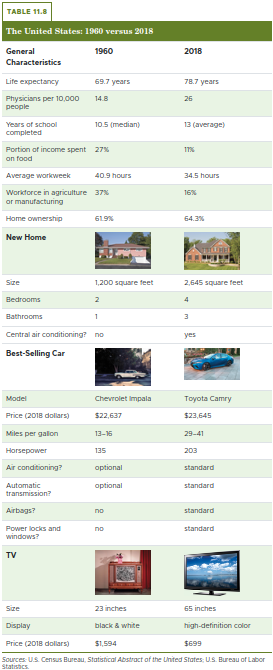
\includegraphics[scale=0.5]{../../images/Chapter 11/Table 11.8.png} This correspond to the page above "%\newpage"
\end{center}

\newpage

\section*{How do resources and technology contribute to economic growth?}
At this point, you may wonder what can be done to provide the best opportunity for economic growth. We see economic growth in many, though certainly not all, nations; but even in those that have grown in the past, future growth is not assured. We now turn to major sources of economic growth.

Economists continue to debate the relative importance of the factors leading to economic growth. However, there is a general consensus on the significance of three factors for economic growth: \textit{resources, technology, and institutions}. In this section, we examine the first two; later in the chapter, we look at institutions.

\end{document}
